\documentclass[../thesis.tex]{subfiles}

\begin{document}

\chapter[Accidental backgrounds, multiplicity cut]{Accidental background rate and multiplicity cut efficiency}
\label{chap:accDMC}
% \chapter*{Accidentals rate and DMC efficiency}
% \stepcounter{chapter}

% XXX this still needs to be updated in some areas to account for our use of a DMC-like isolation cut instead of a symmetric one. Does it? Looks like we updated it.

\def\Emin{\ensuremath{E_\mathrm{min}}} \def\Emax{\ensuremath{E_\mathrm{max}}}
\def\Rs{\ensuremath{R_\mathrm{s}}} \def\Rplu{\ensuremath{R_\mathrm{+}}}
\def\Rpro{\ensuremath{R_\mathrm{p}}} \def\Rdel{\ensuremath{R_\mathrm{d}}}
\def\Rsub{\ensuremath{R_\mathrm{\lambda}}} \def\Nplu{\ensuremath{N_\mathrm{+}}}
\def\Npro{\ensuremath{N_\mathrm{p}}} \def\Ndel{\ensuremath{N_\mathrm{d}}}
\def\eisol{\ensuremath{\epsilon_\mathrm{i}}}
\def\emu{\ensuremath{\epsilon_\mathrm{\mu}}}
\def\etot{\ensuremath{\epsilon_\mathrm{tot}}}
\def\Racc{\ensuremath{R_\mathrm{acc}}}

We combine our discussion of these two quantities because they both depend on the rate of uncorrelated physics events, or \emph{singles.} The accidental background rate (``accidentals rate'') is determined by the probability of two singles occurring in the same coincidence window, while the efficiency of the decoupled multiplicity cut (DMC) is similarly based on the chance of one or more singles occurring within a certain distance in time from the delayed event.\footnote{IBDs and correlated backgrounds also contribute to the inefficiency of the DMC, but the effect is negligible given the vast disparity in rates between singles and correlated events.}

Let $\Rs(\Emin, \Emax)$ be the rate of singles whose reconstructed energy lies between \Emin\ and \Emax. To be precise, \Rs\ is the \emph{true physical rate} of all \emph{muon-uncorrelated} processes that produce such singles. Naively, one could attempt to calculate \Rs\ by counting all non-muon-vetoed triggers in $(\Emin, \Emax)$ and dividing by the veto-corrected DAQ livetime. However, the rate will then be overestimated due to the inclusion of triggers from correlated events, and, likewise, the predicted accidentals spectrum will be distorted.

Instead, the correct approach is to apply an isolation cut (in time) to ensure a clean sample of true singles. A correction must then be applied for the efficiency of this cut. Once \Rs\ has been obtained in this way, calculation of the accidentals rate and DMC efficiency is a straightforward application of Poisson statistics.

\section{Event classes}
\label{sec:accdmcevtcls}

Let us define a \emph{muon-like} event as an AD trigger with charge of at least 3,000 p.e. (about 18~MeV), corresponding to the charge threshold of the AD-muon veto in our IBD selection (\autoref{sec:selMuonVeto})
% \footnote{It would be simpler to define a muon-like event directly in terms of energy instead of charge, but we use 3,000 p.e. for consistency with the historical LBNL analysis. Also, we don't call these events ``muons'', as 3,000 p.e. is not necessarily the definition of an AD muon used in the IBD selection.}
Then a \emph{sub-muon} event is one with reconstructed energy of at least 12~MeV, but not enough charge to be muon-like. A \emph{prompt-like} event has energy of 0.7--12~MeV, a \emph{delayed-like} event 6--12~MeV, and, finally, a \emph{prompt-plus} event is one that is either prompt-like or a sub-muon. The sample described in \autoref{sec:singsel} consists of prompt-plus events.

Similarly, we define the \emph{prompt-like rate} \Rpro\ as $\Rs(0.7, 12)$, the \emph{delayed-like rate} \Rdel\ as $\Rs(6, 12)$, the \emph{sub-muon
  rate}\footnote{$\lambda$ precedes $\mu$ in the Greek alphabet. Right?}
\Rsub\ as $\Rs(12, \sim18)$,\footnote{Technically, we define a sub-muon as an event that has a reconstructed energy above 12~MeV and that is \emph{not classified as muon-like.} Thus an event with an energy slightly above 18~MeV, but a reconstructed charge below the 3,000-PE muon threshold, will be classified as a sub-muon.} and the \emph{prompt-plus rate} \Rplu\ as $\Rpro + \Rsub$. Likewise, the raw event counts in our sample are \Npro, etc. To complete this round of definitions, let \eisol\ be the isolation cut efficiency, \emu\ the muon cut efficiency (for the singles selection), and $T$ be the raw DAQ livetime of the sample.

\section{Singles selection}
\label{sec:singsel}

We begin with a sample of singles. As described in \autoref{sec:selSingles}, these are events that meet the following criteria:

\begin{comment}
  This is the current state of the code:
  \begin{enumerate}
  \item Not a flasher or forced trigger.
  \item Not a muon.
  \item AdSimple energy of at least 0.7~MeV.
  \item No other events passing cuts 1-3 within time window $\pm t$.
  \item Not in a muon veto window.
  \end{enumerate}
  Below is what it should be. Why the difference? XXX Gotta correct for the
  lack-of-muon-vetoing-of-other in dmcEffSingles??? Or enhance the
  SinglesSelector to also pull events from ClusterTree, in case the ``extra'' is
  vetoed (YES, THIS)? We really need to think about whether the events we're
  ``isolating from'' are in the same class as ``this event''. If so then our
  cuts look like(?):
\end{comment}

\begin{enumerate}
\item Not a flasher or forced trigger.
\item Not in a muon veto window.
\item AdSimple energy of at least 0.7~MeV.
\item Charge of less than 3,000 p.e. (i.e., not muon-like)
\item No other such events within 400~\us\ before the event
\item No other such events \emph{between 6 and 12~MeV} within 200~\us\ after the event
\end{enumerate}

The muon veto conditions need not be the same as those used in the IBD selection, as long as they are sufficiently stringent (as explained in \autoref{sec:avoidmuoncorr}). Likewise, the final two conditions (the \emph{isolation cut}) can be chosen somewhat arbitrarily, provided that the window is large enough to remove correlated triggers and small enough to provide sufficient statistics. The actual employed isolation cut is designed to mimic the IBD selection's multiplicity cut as closely as possible, as discussed in \autoref{sec:selSingles}.

\section{Muon veto considerations}
\label{sec:muonventoconsider}

\subsection{Avoiding muon-correlated events}
\label{sec:avoidmuoncorr}

In the selection criteria described in \autoref{sec:singsel}, the final one (the isolation cut) requires ``no other events passing the above cuts within time window $\pm t$''. Since ``the above cuts'' includes ``not in a muon veto window'', this implies that an extra \emph{muon-correlated} trigger will \emph{not} lead to event rejection by the isolation cut.

This formulation of the isolation cut is necessary for the mathematical consistency of the calculation of its efficiency: We will be assuming that the events we are measuring---muon-uncorrelated singles---belong to the exact same class as the ``extra'' events that enter the definition of the isolation cut.

However, at first glance this poses a problem: Our goal is to measure muon-uncorrelated events, but if we allow a potential ``single'' to be preceded by a muon-correlated trigger, then the ``single'' may itself be the product of muon activity.

Fortunately, this problem can be easily eliminated by an appropriate choice of the muon veto window. In particular, we need to ensure that, if there is a muon-correlated event lying inside the isolation window preceding a singles candidate, the same muon \emph{will veto our candidate}. Previous studies have shown that the majority of muon-induced activity occurs within 400~$\mu$s of the muon. Therefore, if we veto at least $t$ + 400~$\mu$s after a muon (where $t$ is the length of the isolation cut window), the presence of a muon-correlated trigger guarantees that the candidate will get rejected, albeit by the muon veto, not by the isolation cut. During singles selection, therefore, we are careful to use muon veto windows that are sufficiently long.

\subsection{Decoupling of efficiencies}
\label{sec:effdecoup}

\def\Pa{\ensuremath{P_\mathrm{a}}} \def\Pb{\ensuremath{P_\mathrm{b}}}
\def\Pab{\ensuremath{P_\mathrm{ab}}}

In the calculations that follow, we assume that
\begin{equation}
  \label{eq:effdecoup}
  \etot = \emu \eisol,
\end{equation}
that is, that we can calculate the muon veto and isolation cut efficiencies independently, and get the total efficiency by multiplying the two. This assumption is valid only if the two occurrences---either a muon, or an ``extra'' single---are statistically independent. As was explained above, extra muon-correlated triggers are \emph{not} considered when applying the isolation cut. Therefore, the presence of a muon has no effect on the probability of passing the isolation cut, and, conversely, the presence of an extra uncorrelated single has no effect on the probability of being inside a muon veto window. The requirements for statistical independence are thus satisfied.

As a final verification of \autoref{eq:effdecoup}, let us divide rejected events into three non-overlapping categories: (a), events rejected only by the muon veto, (b), events rejected by the isolation cut, and (ab), events rejected by both. Since the two cuts are independent, $\Pab = \Pa\Pb$. We have:
\begin{align*}
  \etot &= 1 - \Pa - \Pb - \Pab \\
        &= 1 - (1-\emu)\,\eisol - \emu\,(1-\eisol) - (1-\emu)(1-\eisol) \\
        &= \emu \eisol
\end{align*}
Clearly, \autoref{eq:effdecoup} indeed applies. The muon veto efficiency is determined simply by keeping track of the total vetoed livetime, while the isolation cut efficiency is described next.

% XXX 200 us or 400 us or...?

\section{Isolation cut efficiency}
\label{sec:isolcuteff}

\newcommand\NL{\ensuremath{N_{\mathrm{L}}}}
\newcommand\RL{\ensuremath{R_{\mathrm{L}}}}
\newcommand\tL{\ensuremath{t_{\mathrm{L}}}}
\newcommand\NR{\ensuremath{N_{\mathrm{R}}}}
\newcommand\RR{\ensuremath{R_{\mathrm{R}}}}
\newcommand\tR{\ensuremath{t_{\mathrm{R}}}}

Let ``L'' and ``R'' (i.e. left and right) refer to the two classes of events that would lead to rejection of a singles candidate, should such an event be measured within a time window of (respectively) $\tL$ before or $\tR$ after the candidate. Let $\NL$ and $\RL$ denote, respectively, the raw measured count and the true rate of L-class events, and likewise for $\NR$ and $\RR$. Also let $T$ denote the total livetime.

As a starting point, we have the following identities:
\begin{align}
  \label{eq:ident0}
  \begin{split}
    \NL &= \emu \eisol \RL T \\
    \NR &= \emu \eisol \RR T
  \end{split}
\end{align}
in which \emu\ and $T$ and each $N$ are known, while the unknowns are \eisol\ and each $R$. In addition, the Poisson distribution implies that
\begin{equation}
  \label{eq:ident1}
  \eisol = e^{-\RL \tL -\RR \tR}.
\end{equation}
This is simply the probability of observing zero L-class events in a time window of length $\tL$, and zero R-class events in a $\tR$-length window. Combining \autoref{eq:ident0} and \autoref{eq:ident1}, we have:
\begin{align*}
  \begin{split}
    \NL &= \emu e^{-\RL \tL -\RR \tR} \RL T \\
    \NR &= \emu e^{-\RL \tL -\RR \tR} \RR T \\
\end{split}
\end{align*}
or, after rearranging and multiplying the top and bottom equations by $\tL$ and $\tR$, respectively,
\begin{align*}
  \begin{split}
    e^{\RL \tL + \RR \tR} \NL \tL &= \emu \RL \tL T \\
    e^{\RL \tL + \RR \tR} \NR \tR &= \emu \RR \tR T. \\
  \end{split}
\end{align*}
Adding these two coupled equations gives
\begin{equation}
  e^{\RL \tL + \RR \tR} (\NL \tL + \NR \tR) = \emu (\RL \tL + \RR \tR) T
\end{equation}
which, after some rearrangement, gives:
\begin{equation}
  (-\RL \tL - \RR \tR) e^{-\RL \tL - \RR \tR} = -\frac{\NL \tL + \NR \tR}{\emu T}.
\end{equation}
This equation takes the form $we^w = z$, which cannot be solved for $w$  using elementary functions. Instead we employ the Lambert $W$ function, defined as the inverse of the map $w \mapsto we^w$ (that is, $W(we^w) = w$). As shown in \autoref{fig:lambertW}, the $W$ function has two branches. We know that, for an O(1~ms) isolation window, $\RL \tL \ll 1$ (and likewise for $\RR$), implying that the correct choice is the upper branch $W_0$. Then
\begin{equation}
  % \Rplu = -\frac{1}{2t}\, W_0 \left(-\frac{2\Nplu t}{\emu T}\right).
  \RL \tL + \RR \tR = - W_0\left(-\frac{\NL \tL + \NR \tR}{\emu T}\right)
\end{equation}
Finally, inserting this into \autoref{eq:ident1}, we obtain the isolation cut
efficiency:
\begin{equation}
  \label{eq:accIsolEff}
  \eisol = \exp \, W_0 \left( -\frac{\NL \tL + \NR \tR}{\emu T} \right).
\end{equation}

\begin{figure}
  \centering 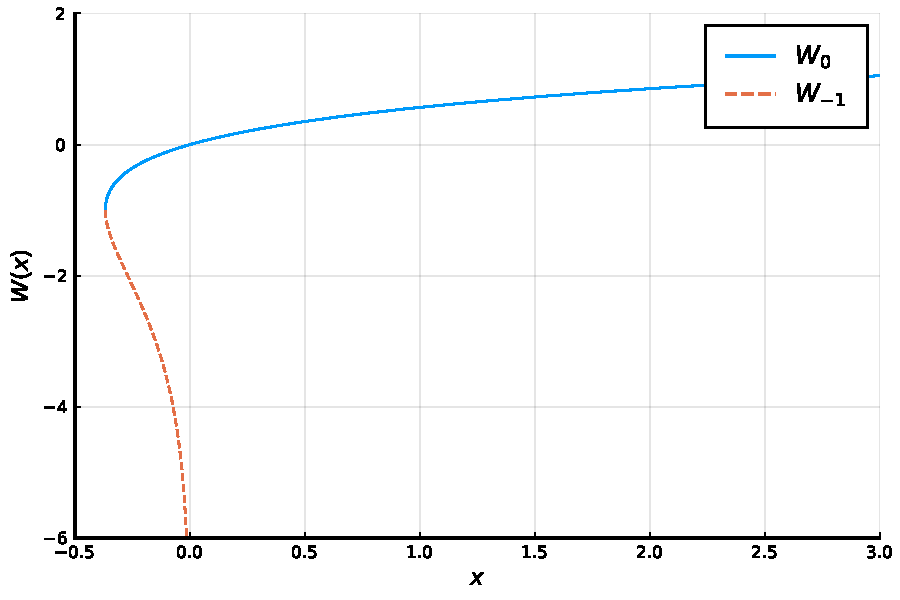
\includegraphics[scale=0.7]{AccAndDMC/lambertW.pdf}
  \caption{The two branches of the Lambert $W$ function.}
  \label{fig:lambertW}
\end{figure}

\section{Singles rates}
\label{sec:singratescalc}

Once the isolation cut efficiency is known, it is trivial to calculate the prompt- and delayed-like singles rates:
\begin{equation}
  \label{eq:accSingRates}
  \Rpro = \frac{\Npro}{\eisol \emu T},\qquad
  \Rdel = \frac{\Ndel}{\eisol \emu T},
\end{equation}
and so on. These quantities are essential for calculating the DMC efficiency and accidentals rate, as described below.

\section{DMC efficiency}
\label{sec:dmceffcalc}

\def\edmc{\ensuremath{\epsilon_\mathrm{m}}}

In order for an IBD candidate to satisfy the decoupled multiplicity cut, there must be no delayed-like triggers in the 200~$\mu$s following the delayed event, and no extra prompt-plus events\footnote{Formerly, in the LBNL analysis, only extra \emph{prompt}-like events would lead to a DMC rejection. In order to
  eliminate the double neutron background, ``prompt-like'' was later changed to
  ``prompt-plus''.} in the 400~$\mu$s prior to the delayed event. More formally,
\begin{align}
  \edmc &= P(0; \Rplu \cdot 2\tau)\;P(0; \Rdel \cdot \tau) \nonumber \\
        &= \exp [-(2\Rplu\tau + \Rdel\tau)],
          \label{eq:dmcEff}
\end{align}
where $\tau$ = 200~$\mu$s.

\section{Accidentals rate}
\label{sec:accratecalc}

\subsection{Rate calculation}
\label{sec:accRateCalc}

An accidental event, in order to enter the IBD selection, must pass the DMC, as with any other IBD candidate. Since the DMC is ``centered'' on the delayed event of the pair, it is simplest to calculate the accidentals rate by similarly centering the calculation on the delayed event.

Given an uncorrelated delayed-like trigger, we can calculate the probability that it forms the delayed half of an accidental IBD candidate. Letting all time intervals be defined in relation to the delayed-like trigger, there are four conditions:
\begin{enumerate}
\item Exactly one prompt-like event in [-200, 0]~$\mu$s.
\item No sub-muon events in [-200, 0]~$\mu$s.
\item No prompt-plus (prompt-like or sub-muon) events in [-400, -200]~$\mu$s.
\item No delayed-like events in [0, 200]~$\mu$s.
\end{enumerate}
The accidentals rate is then simply the product of these probabilities multiplied by the delayed-like singles rate:
\begin{align}
  \label{eq:accRate}
  \Racc &= \Rdel \cdot P(1; \Rpro \tau)\cdot P(0; \Rsub \tau)
           \cdot P(0; \Rplu \tau)\cdot P(0; \Rdel \tau) \nonumber \\
        &= \Rdel\cdot\Rpro\tau e^{-\Rpro\tau}\cdot e^{-\Rsub\tau}
           \cdot e^{-\Rplu\tau} \cdot e^{-\Rdel\tau}
\end{align}

Note that this calculation incorporates the inefficiency of the DMC (but not of the muon veto cut). By convention, the oscillation fitter expects background rates to be provided as ``theoretical'' rates, that is, the rate expected if all cuts were perfectly efficient. Internally, the fitter multiplies these rates by the DMC and veto efficiencies. Therefore, we must divide out the DMC efficiency when providing the accidentals rate to the fitter:
\begin{equation}
  \Racc' = \frac{\Racc}{\edmc}.
\end{equation}

\subsection{Statistical uncertainty}
\label{sec:accStatUnc}

The accidentals rate, as calculated using \autoref{eq:accRate}, carries a statistical uncertainty which derives from that of the rates that enter the calculation: the prompt-like rate, delayed-like rate, etc. In turn, these rates, as specified by \autoref{eq:accSingRates}, derive their own uncertainties from those of the event counts in each classification. The uncertainties of the counts are trivial, being merely the Poisson uncertainty of $\sqrt{N}$. However, once we consider the \emph{rates} rather than the \emph{counts}, we begin to encounter complications. Most notably, the isolation cut efficiency $\epsilon_{\mathrm{i}}$ in \autoref{eq:accSingRates} is \emph{also} a function of the event counts, as indicated by \autoref{eq:accIsolEff}. This nonlinear dependence on the event counts is only made more complicated when the rates are inserted into \autoref{eq:accRate}. Furthermore, the event classifications in question are not always statistically independent: For instance, the prompt-like and delayed-like counts are correlated by virtue of the fact that they both include events in the 6--12 MeV region.

In spite of these complications, it is still possible to undertake a theoretical calculation of the statistical uncertainty on the accidentals rate. This would involve expanding \autoref{eq:accRate} in terms of the various event counts $N_{\mathrm{p}}$, $N_{\mathrm{d}}$, etc., and then re-expressing the event counts (such as the prompt-like and delayed-like counts) as sums of counts of \emph{disjoint} event classes $N_1$, $N_2$, etc. (e.g., an 0.7--6 MeV class and a 6--12 MeV class). This complicated function $R_{\mathrm{acc}}(N_1, N_2, \ldots)$ could then be expanded in a power series using computer algebra. From that, an expression for the variance $\braket{R_{\mathrm{acc}}^2} - \braket{R_{\mathrm{acc}}}^2$ could be obtained up to any desired order, and evaluated using the known cumulants of the Poisson distribution.

Given the complexities of this procedure, and the fact that previous studies have established this statistical uncertainty to be significantly smaller than the systematic uncertainty, the author has no desire to pioneer such an undertaking. Nevertheless, it remains desirable to have some way of evaluating the statistical uncertainty in order to verify its relative insignificance.
% , particularly when the prompt and/or delayed energy cuts are loosened enough to significantly increase the accidentals rate.
For this reason, a simple Monte Carlo procedure was developed for calculating this uncertainty. We proceed to discuss its implementation and results.
% It gave results consistent with the uncertainty published in \cite{An_2017}. (TODO: Include details; show my histogram of accidentals rates under random variations of the prompt/delayed-like rates.)

\subsubsection{Procedure}
\label{sec:accStatUncProc}

To recap, only three inputs are required to calculate the accidentals rate:
\begin{itemize}
\item The livetime.
\item The muon veto efficiency (for correcting the livetime).
\item The energy histogram of all events selected by the singles selection.
\end{itemize}
In turn, to study the statistical uncertainty $\sigma$ of the calculation, we can apply statistical fluctuations to the energy histogram. These fluctuations will automatically propagate to the event counts $N_p$, etc., and then to the final result. Repeating this procedure will produce a sample of accidentals rates, from which $\sigma$ can be determined by taking the standard deviation or by fitting a Gaussian function.

For each bin $i$ of the singles' energy histogram, with measured count $\overline{N}_i$, let $N_i$ denote corresponding the random variable describing a hypothetical ensemble of experiments. The PDF $f(N_i)$ is then given by the Poisson distribution:
\begin{equation}
  f(N_i) = \frac{\overline{N}_i^{N_i}e^{-\overline{N}_i}}{N_i!}.
\end{equation}
This distribution is sampled for each bin, resulting in a fluctuated singles histogram, which is then used as the input for the calculation of the accidentals rate described in \autoref{sec:accRateCalc}. We repeat this procedure 10,000 times for each AD (and data period) in order to obtain a sample of accidentals rates that approximates their statistical distribution, as illustrated in \autoref{fig:acc_stat_unc_hist}. Finally, the statistical uncertainty is determined from this distribution in two ways: First, by directly calculating the standard deviation, and second, by performing a fit to a Gaussian function. Both methods produce consistent results.

As shown in Figures~\ref{fig:acc_stat_unc_prd6}--\ref{fig:acc_stat_unc_prd0}, the statistical uncertainty of the accidentals rate is relatively small, remaining below the 1\% level even in the lowest-statistics case (EH3 in the 7AD period). Rather than using these uncertainties directly, we absorb them into a conservative 2\% total uncertainty in order to account for possible systematic effects, as discussed in \autoref{sec:accSystUnc}.

\begin{figure}[ht]
  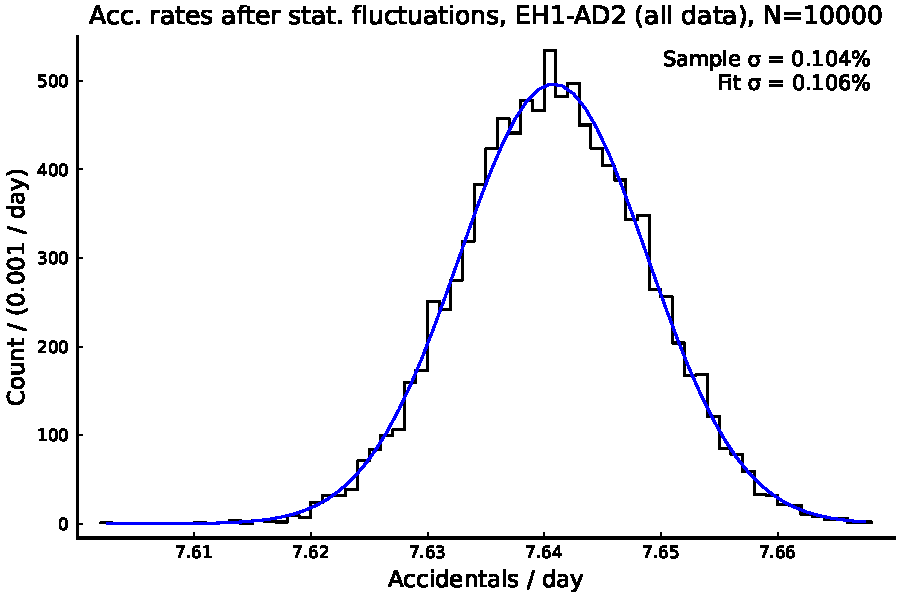
\includegraphics[width=0.7\textwidth]{AccAndDMC/acc_stat_unc_hist_eh1ad2_all.pdf}
  \caption{Distribution of full-dataset accidentals rates in EH1-AD2 calculated under statistical fluctuations of the singles rate and spectrum. Consistent estimates of the spread are obtained from directly calculating the standard deviation and from performing a fit to a Gaussian function.}
  \label{fig:acc_stat_unc_hist}
\end{figure}

\begin{figure}[ht]
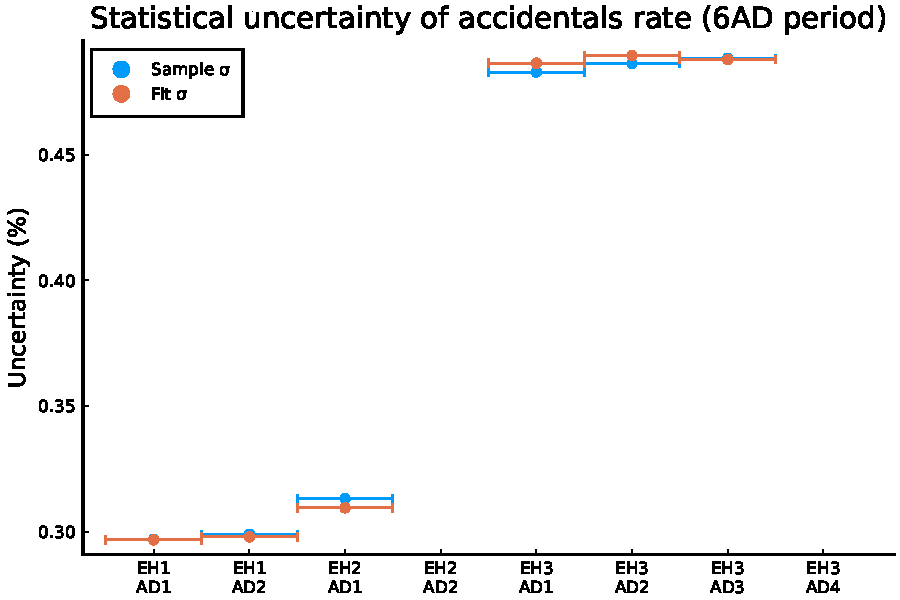
\includegraphics[width=0.7\textwidth]{AccAndDMC/acc_stat_unc_prd6.pdf}
\caption{Statistical uncertainty of the accidentals rates in each AD for the 6AD period. ``Samples $\sigma$'' refers to the directly-calculated standard deviation, while ``Fit $\sigma$'' refers to the results of fitting to a Gaussian function.}
\label{fig:acc_stat_unc_prd6}
\end{figure}

\begin{figure}[ht]
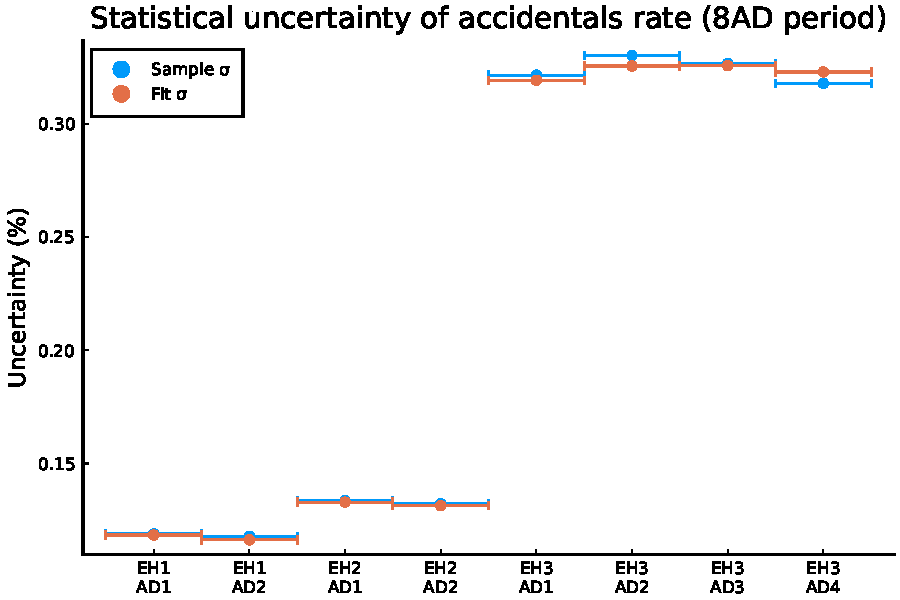
\includegraphics[width=0.7\textwidth]{AccAndDMC/acc_stat_unc_prd8.pdf}
\caption{Statistical uncertainty of the accidentals rates in each AD for the 8AD period. ``Samples $\sigma$'' refers to the directly-calculated standard deviation, while ``Fit $\sigma$'' refers to the results of fitting to a Gaussian function.}
\label{fig:acc_stat_unc_prd8}
\end{figure}

\begin{figure}[ht]
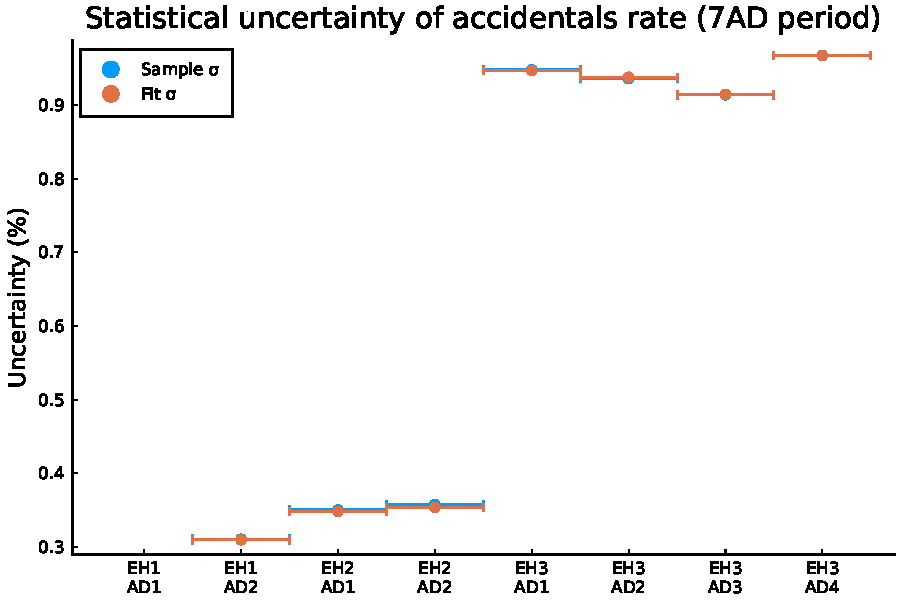
\includegraphics[width=0.7\textwidth]{AccAndDMC/acc_stat_unc_prd7.pdf}
\caption{Statistical uncertainty of the accidentals rates in each AD for the 7AD period. ``Samples $\sigma$'' refers to the directly-calculated standard deviation, while ``Fit $\sigma$'' refers to the results of fitting to a Gaussian function.}
\label{fig:acc_stat_unc_prd7}
\end{figure}

\begin{figure}[ht]
  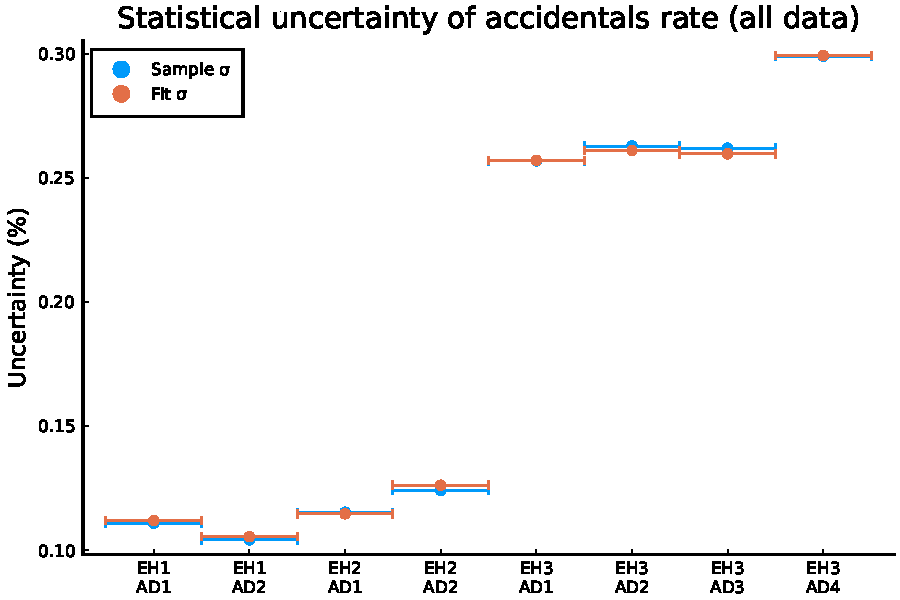
\includegraphics[width=0.7\textwidth]{AccAndDMC/acc_stat_unc_prd0.pdf}
  \caption{Statistical uncertainty of the accidentals rates in each AD for the full dataset. ``Samples $\sigma$'' refers to the directly-calculated standard deviation, while ``Fit $\sigma$'' refers to the results of fitting to a Gaussian function.}
  \label{fig:acc_stat_unc_prd0}
\end{figure}

\subsection{Systematic and total uncertainty}
\label{sec:accSystUnc}

The systematic uncertainty on the accidentals rate can be estimated by comparing our method to an independent technique. Rather than carrying this out ourselves, we refer to previous studies that performed such comparisons \cite{An_2017}. In those studies, the alternative calculations used the so-called \emph{offset-window} method, in which the IBD selection is repeated with the requirement of a time offset (ranging from 1 to 20~ms) between the prompt and delayed triggers. This offset has the effect of largely eliminating correlated events, producing a sample enriched in accidentals. From this sample, one can obtain the distribution of the spatial separations between the prompt and delayed triggers in each pair. Finally, for the true IBD sample, the prompt-delayed distribution can be plotted, and the distribution for the accidental sample can be normalized to fit it, giving an estimate of the total number of accidentals in the true sample (\autoref{fig:accOffsetWindow}). This method was shown to give consistent results with methods based on measuring the singles rates (such as our method), with a slightly higher statistical uncertainty of about 1\%. To obtain our own final uncertainty on the accidentals rate, we take this 1\% and conservatively add it linearly to our own 1\% worst-case statistical uncertainty, giving 2\%. Although this is an overestimate, it has a minimal effect on the final uncertainty of the oscillation parameters, given that the total background uncertainty remains dominated by $^9$Li/$^8$He.

\begin{figure}[ht]
  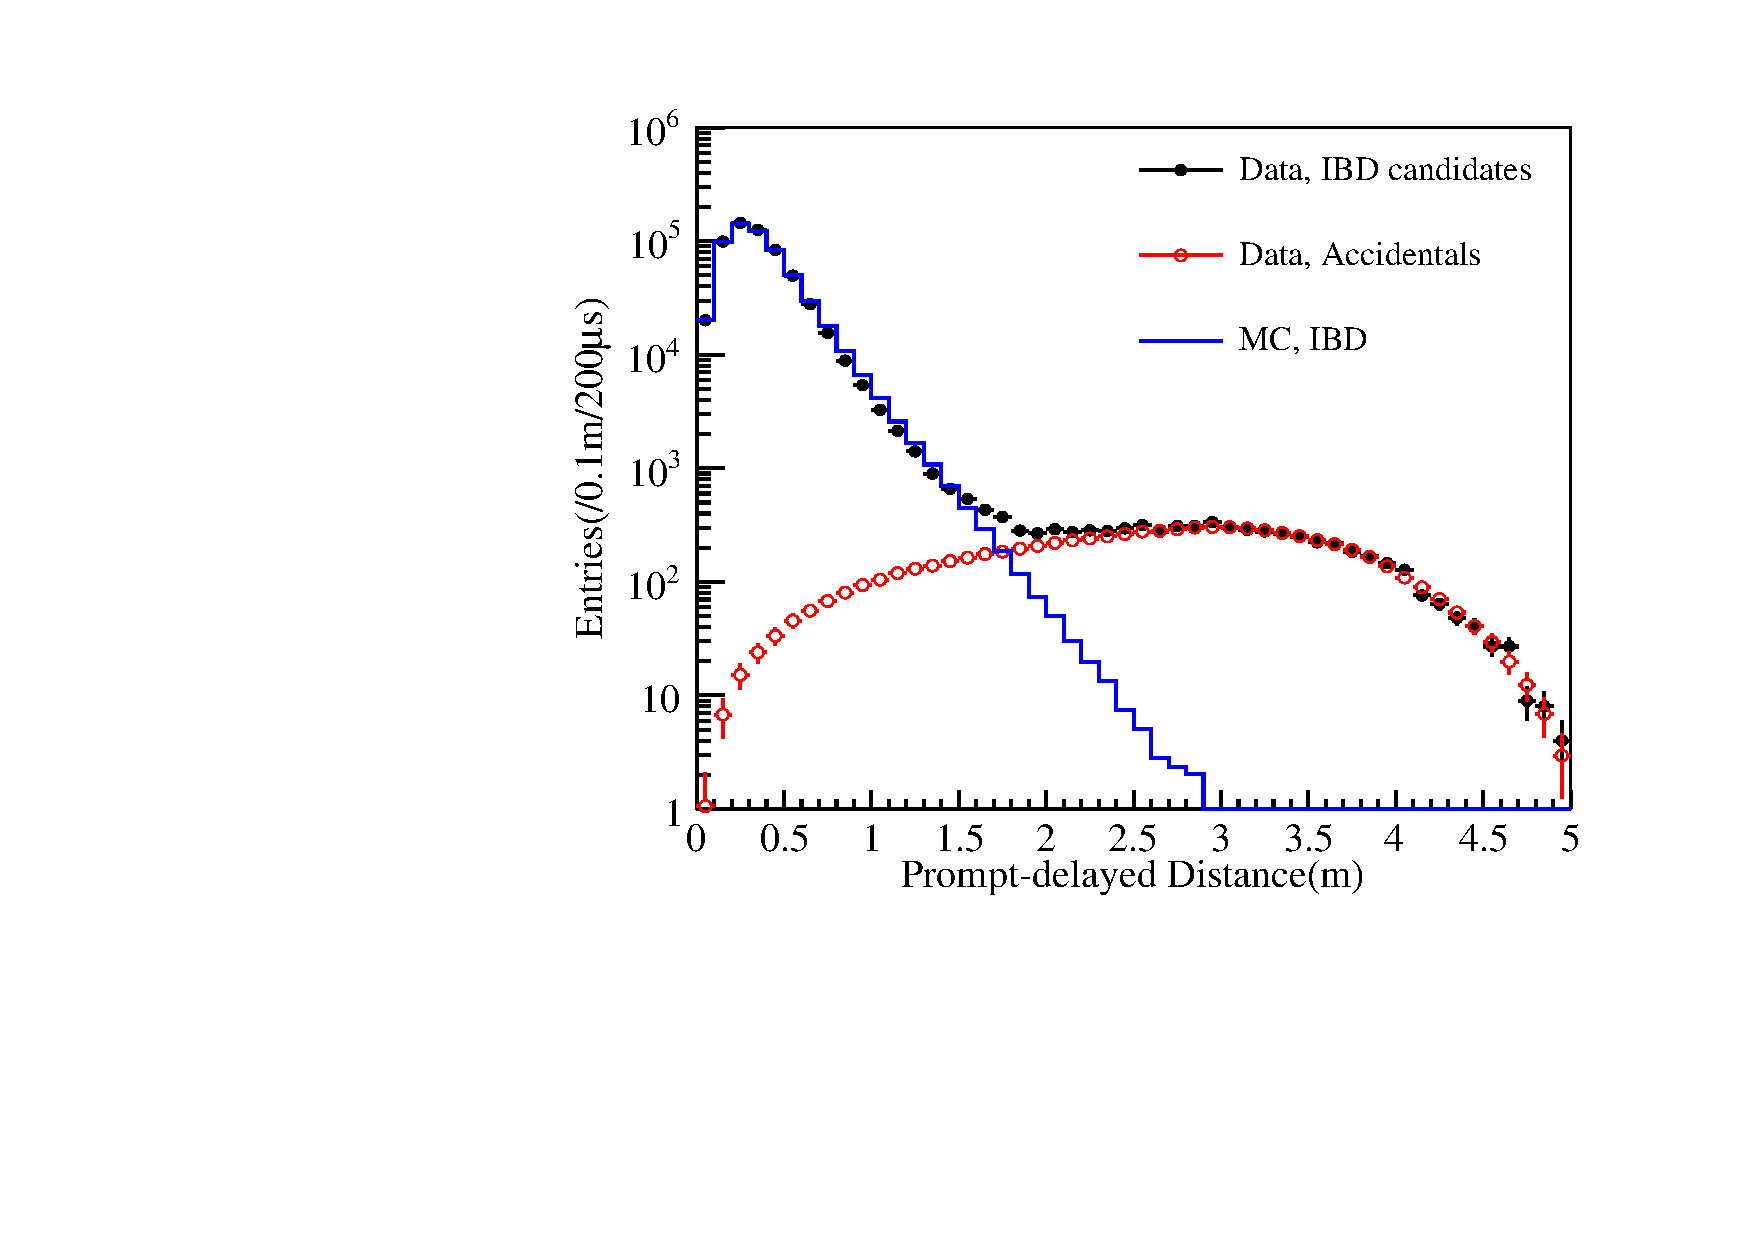
\includegraphics[width=0.7\linewidth]{AccAndDMC/evt_acc_distance.pdf}
  
  \caption{Distribution of prompt-delayed distances for a true IBD sample and for an accidentals-enriched sample, as obtained when using the offset-window method of measuring the accidentals rate. The particular AD shown is unspecified. From \cite{An_2017}.}
    \label{fig:accOffsetWindow}
\end{figure}

% \section{Conclusions}
% \label{sec:accdmcconcl}

% The most subtle part of this calculation is the efficiency of the isolation cut.
% I hope that there isn't any circular logic lurking in my derivation.

\end{document}
